\documentclass[conference]{IEEEtran}
\usepackage{amsmath,amssymb,graphicx,booktabs,url,xcolor}
\usepackage{tikz}
\usetikzlibrary{arrows.meta,positioning}
\title{GNSS Re-entry with LiDAR--Inertial Odometry: A Prospective Study of Timeliness--Accuracy Tradeoffs}
\author{\IEEEauthorblockN{Internal author-review draft: authors and affiliations unassigned}}
\newcommand{\reviewmark}{\textcolor{red}{\textbf{NOT\_SUBMISSION\_READY: author approval and venue checks pending.}}}
\begin{document}\maketitle
\begin{center}\small\reviewmark\end{center}
\begin{abstract}
Returning GNSS can be available before a position filter should use it. We study actual update delay, exposure to artificially biased observations and position error in a common filter propagated by FAST-LIO2 relative motion. An unchanged motion-and-anchor recovery manager is compared with direct fusion, innovation gates, Huber weighting, seven qualification durations and ablations. After development and retrospective evaluation on two seen routes, the full source, inputs, clock, cache and nineteen policies were frozen, pushed and verified before opening a third route. Its 152 matched runs cover natural data and seven fixed perturbation categories, without new-route tuning. On a prospectively frozen building01 route, P fails the joint service, natural-cost and coverage gate. Its biased post90 error is 2.378m; the strongest eligible alternative, B3, gives 4.0299m. A long wait may attain lower error while violating timely clean re-entry. The prospective route does not support the preregistered joint claim: biased-return error decreases, but the natural-cost cap is violated. The evidence is a conditional tradeoff and failure boundary, not a compliant superiority claim. Reference states beyond a declared common initial condition are used only offline. Controlled bias exposure and cached-clock bounds are not field fault probabilities or live end-to-end latency.
\end{abstract}
\begin{IEEEkeywords}GNSS recovery, LiDAR--inertial odometry, observation admission, latency, prospective evaluation\end{IEEEkeywords}

\section{Introduction}
A robot can continue navigating with LiDAR--inertial odometry (LIO) during a GNSS outage, but returning receiver positions pose a different question: when should they resume correcting global position? Immediate updates can propagate biased observations. Long waits can avoid them while delaying useful corrections and allowing local drift to grow. Accuracy depends on selection, timeliness and the evaluation horizon.

Under a finite artificial bias, a controller may reject GNSS until the bias disappears and obtain low error without timely correction when unchanged observations return. Conversely, admitting fewer injected rows need not reduce actual error: their displacement can cancel receiver error. Neither RMSE nor exposure alone measures recovery quality.

We evaluate an existing motion-and-anchor manager in a shared outer position filter. The specific question is whether it improves biased-return error against complete simple controls under a 15-s clean-update deadline, a natural-cost cap and full coverage. The service protocol was formulated after R1 outcomes; building00 development and parking00 retrospective results are seen evidence. building01 is a new prospective test with unchanged parameters and a verified remote scientific freeze before precision access.

The contribution is an auditable empirical study separating actual updates from state transitions and offline error recovery, with full waits, strict NIS, ablations and a new-route boundary. FAST-LIO2, KF-GINS and the recovery components retain their original attribution. No new 21-dimensional filter, mechanism revision, field multipath detector or universal superiority is claimed.
\section{Related Work}
FAST-LIO2 estimates local motion through direct LiDAR--inertial estimation~\cite{fastlio2}. We use the fixed i2Nav AT128/ADIS adaptation, rather than modifying its point-cloud estimator. KF-GINS implements a separate 21-dimensional GNSS/INS error-state filter~\cite{kfgins}; its posterior is not fed repeatedly into the three-dimensional filter studied here. Huber's robust estimation~\cite{huber} motivates a standard covariance-weighting comparator; innovation gating provides another simple selection rule.

WinTA-GIL~\cite{winta} uses windowed trajectory matching and motion/quality-triggered heading refinement, feeding optimized heading into an EKF. Our implementation keeps its initial local-to-NED alignment fixed and manages receiver-position admission. This scope difference is not a novelty proof: motion windows and recovery-triggered consistency already have precedent.

Dual-ACKF~\cite{dual} combines an explicit GNSS bias state, innovation-based covariance adaptation, robust updates, and recovery protection. Our availability-based control uses the same outer position KF as every other policy; it is not a reproduction of the full Dual-ACKF system. Neither Dual-ACKF nor WinTA-GIL was executed in this benchmark, and their published accuracy is not inserted into our comparison tables. Their mechanisms constrain what this study can claim as original.

\section{Common Filter and Existing Recovery Policy}
\subsection{Shared Estimator}
\begin{figure}[t]
\centering
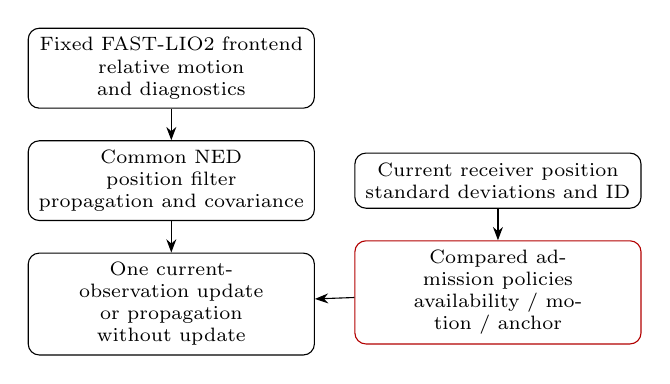
\begin{tikzpicture}[node distance=4mm,every node/.style={draw,rounded corners,font=\scriptsize,align=center,text width=34mm,minimum height=7mm},>=Stealth]
\node (lio) {Fixed FAST-LIO2 frontend\\relative motion and diagnostics};
\node[below=of lio] (prop) {Common NED position filter\\propagation and covariance};
\node[right=5mm of prop] (gnss) {Current receiver position\\standard deviations and ID};
\node[below=of gnss,draw=red!70!black] (manage) {Compared admission policies\\availability / motion / anchor};
\node[below=of prop] (update) {One current-observation update\\or propagation without update};
\draw[->] (lio)--(prop);\draw[->] (prop)--(update);\draw[->] (gnss)--(manage);\draw[->] (manage)--(update);
\end{tikzpicture}

\caption{Executed framework. Only the admission policy varies. Reference states initialize the declared common condition and support offline evaluation; they never enter the manager. KF-GINS remains an independent comparator.}
\label{fig:framework}
\end{figure}
The state is position $p\in\mathbb{R}^{3}$ in NED, with a common initial alignment $A$. For LIO displacement $\Delta\ell_k$,
\begin{align}
 p_k^-&=p_{k-1}^++A\Delta\ell_k,\\
 P_k^-&=P_{k-1}^++\operatorname{diag}(1,1,4)q_k,\\
 q_k&=0.001\Delta t+0.001\|\Delta\ell_k\|.
\end{align}
The coefficients have units $\mathrm{m^2/s}$ and $\mathrm{m^2/m}$. The antenna observation is $z_k=p_k+R_{NB,k}b+v_k$, with FRD lever arm $b=[0,-0.07,-0.365]^\top$ m. Receiver NED standard deviations are floored at $[1,1,2]$ m before squaring to form covariance $R_k$. For an admitted observation,
\begin{align}
 r_k&=z_k-p_k^--R_{NB,k}b,\\
 K_k&=P_k^-(P_k^-+\bar R_k)^{-1},\\
 p_k^+&=p_k^-+K_kr_k,
\end{align}
with Joseph covariance update and policy-inflated $\bar R_k$. Every original receiver ID is consumed once, including rejected observations. Monitoring differences and historical anchors are not independent position measurements.

\subsection{Motion and Historical Anchor}
With receiver position $z$ and independent LIO antenna position $a$, a five-second window checks
\begin{align}
 d_{ik}&=(z_k-z_i)-(a_k-a_i),\\
 s_{ik}&=d_{ik,xy}^{\top}(R_{k,xy}+R_{i,xy}+q_{ik}I)^{-1}d_{ik,xy}.
\end{align}
The existing P-r03 policy requires an engineering score at most four for two seconds when a motion qualification applies. This score is not a calibrated chi-square test. Gaps greater than 1.5 s clear the monitoring window. An availability shadow policy isolates an anomaly or a GNSS gap greater than two seconds, with a two-second minimum wait and a covariance multiplier initially 15, relaxing over 15 s.

A historical anchor stores the latest raw GNSS observation that was admitted in NORMAL state with valid local diagnostics, acceptable motion score and nominal innovation, continuously qualified for five seconds. During outage recovery it compares
\begin{equation}
 e_k=z_k-\{z_a+(a_k-a_a)\}
\end{equation}
against receiver covariance plus accumulated process covariance. Its horizontal score limit is four. Only an actual GNSS gap activates this anchor check; isolation freezes anchor promotion. Invalid local evidence falls back to the mature availability policy and is logged as unresolved, not as proof of sensor correctness. The two cached interpolation endpoints must have at least 100 effective points and mean absolute plane residual at most 0.2 m for local health eligibility.

This policy cannot distinguish all LIO drift from GNSS bias. A stale or biased anchor can veto useful GNSS; fallback can admit injected observations. There is no bias-state estimation, optimized heading update, or integrity guarantee. The fixed implementation is inherited from R1 rather than revised to fit the R2 results.


\section{Data and Prospective Protocol}
\subsection{Inputs, Roles and Initialization}
The i2Nav-Robot dataset~\cite{i2nav} supplies AT128 LiDAR, ADIS16465 increments, F9P positions and local-NED MM/INS reference. building00 is seen development; parking00 is seen retrospective; building01 is the prospective route. Upstream versions remain fixed: dataset\texttt{2ffdca6d}, adaptation\texttt{6c602f8d}, KF-GINS\texttt{8291a93e}. Its five required originals were streamed/hashed read-only; building01.bag matches the official digest. Text hashes are local identities, not unpublished official checksums. Extra original files were preserved.

Standard/custom IMU headers and custom week/SOW independently establish GPS week 2364 and GPS minus UTC 18 s. All raw texts, including the eight-column trajectory, use SOW. The two IMU streams begin at different rows and are matched by timestamp, not row index. Custom increments match ADIS text; they are angle/velocity increments, not rates to be multiplied by dt again. F9P header precision differs from its three-decimal text within the serialization half-step; backend observations are unchanged. One full 1$\times$ FAST-LIO replay in the existing isolated Noetic runtime produces15245 poses without reference comparison. No cache was chosen by accuracy.

All policies share initialization, cache, covariance, lever arm and observed GNSS timeline. One fixed first reference row supplies the controlled initial position, velocity and attitude; later reference values are offline only. Alignment is fixed, not fitted to each method. The unavailable absolute local origin limits results to initialization-conditioned errors. MM/INS reference shares AT128 map-matching information and is not independent of all sensing.

The complete new-route freeze archives scientific source/tests, all nineteen configurations, calibration, runtime/binary/cache, raw identities, time conversion, unique initialization, all fixed events and metric definitions. Its Git commit was pushed and the exact remote SHA verified before the first152-pair opening. R2's analysis-only archive was not used as authorization. R1/R2 code, failures, numeric logs and paper versions remain intact. A known 3.6013-m RMS discrepancy between two earlier same-bag frontend runs is disclosed; the second building00 cache remains sensitivity, not another route. Only one building01 frontend was preregistered.

\subsection{Fixed Matched Controls}
B2 is LIO-only; B3 direct fusion; B4 the R1-selected NIS100; B5 Huber2.5; B6 availability wait with covariance protection. Clock2/5/10/15/30/60/90 disable motion and anchor veto while retaining the same availability foundation and weighting. Their numbers are qualification durations, not total update delays: the five-second monitoring window adds time. Clock2 equals the time-only ablation. Strict NIS11.3449/16.2662/30 retain the original screened thresholds, without new-route selection. P-no-motion equals B6; P-no-anchor and P-no-decay remove the respective components. These are 19 named policies, including declared aliases, not 19 original algorithms. The inherited local-health fallback can bypass long qualification; a Clock duration is not an unconditional quarantine. Every alternative is shown even when outside the budget.

\subsection{Events, Clocks and Complete Coverage}
At fixed 150/450/750-s offsets with N/E/NE directions, seven categories retain three events each: single 3-m jump, clustered 10-m jumps, 30/60-s deletions with unchanged return, 30-s deletions followed by 3/10-m biases held for 90 s, and a 10-m ramp. Natural data is the eighth case. All 21 events were checked against input/reference time support before precision, including full 180-s post-return windows. No event was moved or removed according to method error.

$t_{return}$ is the first actually present measurement after deletion; $t_{admit}$ is the first logged\texttt{accepted=true} KF update. Admission is right-censored at 180 s. The primary service gate is clean measurement-time delay$\leq15$s, inclusive with$10^{-8}$-s tolerance. Cache-availability upper bounds are reported separately; neither is measured live receiver-arrival latency. Sensitivity budgets are 5/10/30/60/90 s. Offline error recovery is error below 3 m sustained for 5 s within 90 s and can precede any accepted update.

The primary error is the equal-weight mean of three biased post90 horizontal RMSEs after a 30-s deletion and 90-s 10-m bias. All 10/30/60/90/180-s windows use the full common 10-Hz input/reference grid; expected counts, missing coverage and censoring are retained, not successful-only intersections. The natural gate is the best frozen B4/B5/B6 whole-route RMSE plus$\max(2\%,0.05\,\mathrm{m})$. Qualification also requires complete coverage. Injected accepted/exposed counts are computed over exact artificial row IDs, never fed to the manager. All categories, P95/Max and per-event records remain in the evidence package.

\section{Results}
\begin{table*}[t]\centering\small
\caption{Complete prospective building01 matrix: all19 fixed named policies. Horizontal RMSE is meters; clean delay is the maximum of three actual-update measurement delays, seconds. Exposure is accepted/exposed artificial10-m rows. Q requires the frozen15-s clean deadline, natural-cost cap and complete coverage. C180 is right-censored admission, not zero delay. No new-route tuning.}\label{tab:primary}
\begin{tabular}{lrrrrrrc}\toprule
Policy & Natural & Clean delay & Clean90 & Bias90 & Bias180 & Exposure & Q\\\midrule
LIO only & 8.405 & C180 & 1.325 & 1.325 & 1.742 & 0/270 & no \\
Direct fusion & 4.909 & 0.000 & 2.319 & 4.030 & 3.585 & 270/270 & yes \\
NIS100 & 4.956 & 0.000 & 2.319 & 4.030 & 3.585 & 270/270 & yes \\
Huber2.5 & 5.149 & 0.000 & 2.302 & 3.782 & 3.498 & 270/270 & no \\
Availability B6 & 5.252 & 2.000 & 2.338 & 3.182 & 3.333 & 262/270 & no \\
NIS11.3449 & 5.398 & 0.000 & 2.229 & 2.998 & 3.658 & 180/270 & no \\
NIS16.2662 & 5.300 & 0.000 & 2.287 & 2.472 & 2.454 & 180/270 & no \\
NIS30 & 5.079 & 0.000 & 2.313 & 3.170 & 3.598 & 235/270 & no \\
Clock2 & 5.252 & 7.000 & 2.355 & 3.160 & 3.319 & 249/270 & no \\
Clock5 & 5.252 & 10.000 & 2.364 & 3.157 & 3.317 & 240/270 & no \\
Clock10 & 5.252 & 15.000 & 2.376 & 3.140 & 3.306 & 225/270 & no \\
Clock15 & 5.252 & 20.000 & 2.389 & 2.902 & 3.156 & 211/270 & no \\
Clock30 & 5.252 & 35.000 & 2.334 & 2.844 & 3.113 & 183/270 & no \\
Clock60 & 5.252 & 65.000 & 1.973 & 2.368 & 2.358 & 123/270 & no \\
Clock90 & 5.252 & 95.000 & 1.902 & 2.362 & 2.425 & 73/270 & no \\
P-r03 & 5.273 & 7.000 & 2.355 & 2.378 & 2.649 & 166/270 & no \\
P-no-motion & 5.252 & 2.000 & 2.338 & 3.182 & 3.333 & 262/270 & no \\
P-no-anchor & 5.273 & 7.000 & 2.355 & 3.172 & 3.576 & 249/270 & no \\
P-no-decay & 5.177 & 7.000 & 2.342 & 2.388 & 2.532 & 166/270 & no \\
\bottomrule\end{tabular}\end{table*}
\begin{table*}[t]\centering\small
\caption{Cross-route comparison with explicit data roles. All19 policies remain visible. Columns give clean actual-update delay(s), biased post90 horizontal RMSE(m), and joint eligibility Q. building00 is seen development; parking00 is seen retrospective; building01 is the new prospective test. The second building cache is retained sensitivity, not another route.}\label{tab:other}
\begin{tabular}{lrrrrrrrrr}\toprule
 & \multicolumn{3}{c}{Building00: seen development} & \multicolumn{3}{c}{Parking00: seen retrospective} & \multicolumn{3}{c}{Building01: prospective test}\\
Policy & Delay & Bias90 & Q & Delay & Bias90 & Q & Delay & Bias90 & Q\\\midrule
LIO only & C180 & 1.773 & no & C180 & 2.226 & no & C180 & 1.325 & no \\
Direct fusion & 0.000 & 8.371 & yes & 0.000 & 7.015 & yes & 0.000 & 4.030 & yes \\
NIS100 & 0.000 & 8.371 & yes & 0.000 & 3.091 & yes & 0.000 & 4.030 & yes \\
Huber2.5 & 0.000 & 7.645 & yes & 0.000 & 6.426 & yes & 0.000 & 3.782 & no \\
Availability B6 & 2.000 & 5.780 & yes & 2.000 & 4.478 & yes & 2.000 & 3.182 & no \\
NIS11.3449 & 0.000 & 3.653 & no & 0.000 & 2.164 & yes & 0.000 & 2.998 & no \\
NIS16.2662 & 0.000 & 3.700 & no & 0.000 & 2.128 & yes & 0.000 & 2.472 & no \\
NIS30 & 0.000 & 3.908 & no & 0.000 & 2.023 & yes & 0.000 & 3.170 & no \\
Clock2 & 7.000 & 5.558 & yes & 7.000 & 4.395 & yes & 7.000 & 3.160 & no \\
Clock5 & 10.000 & 5.490 & yes & 10.000 & 4.374 & yes & 10.000 & 3.157 & no \\
Clock10 & 15.000 & 5.361 & yes & 15.000 & 4.116 & yes & 15.000 & 3.140 & no \\
Clock15 & 20.000 & 4.899 & no & 20.000 & 3.758 & no & 20.000 & 2.902 & no \\
Clock30 & 35.000 & 4.427 & no & 35.000 & 3.403 & no & 35.000 & 2.844 & no \\
Clock60 & 65.000 & 2.838 & no & 65.000 & 2.521 & no & 65.000 & 2.368 & no \\
Clock90 & 95.000 & 2.510 & no & 95.000 & 2.298 & no & 95.000 & 2.362 & no \\
P-r03 & 7.000 & 3.022 & yes & 7.000 & 2.290 & yes & 7.000 & 2.378 & no \\
P-no-motion & 2.000 & 5.780 & yes & 2.000 & 4.478 & yes & 2.000 & 3.182 & no \\
P-no-anchor & 7.000 & 5.489 & yes & 7.000 & 4.395 & yes & 7.000 & 3.172 & no \\
P-no-decay & 7.000 & 3.059 & yes & 7.000 & 2.259 & yes & 7.000 & 2.388 & no \\
\bottomrule\end{tabular}\end{table*}

\begin{figure*}[t]\centering
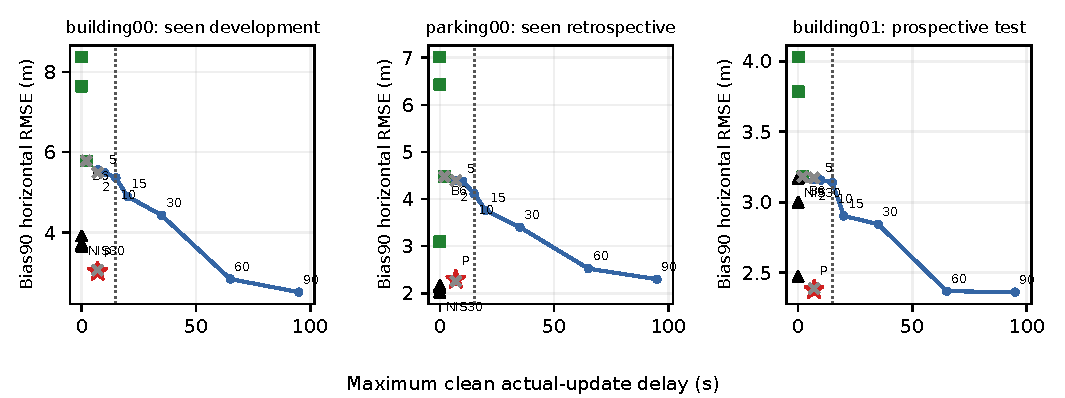
\includegraphics[width=\textwidth]{figures/latency_error_tradeoff.pdf}
\caption{Complete finite-delay policy tradeoffs with explicit route roles. Connected numbers are Clock qualification durations; dotted line is 15-s clean measurement-time budget. Stars are P, black triangles strict NIS, gray crosses ablations. Every policy, including censored B2 and outside-cap controls, remains in Tables~\ref{tab:primary}--\ref{tab:other}; second-cache sensitivity is retained separately. Each panel has its own vertical scale.}
\label{fig:tradeoff}\end{figure*}

\subsection{Prospective Completeness and Main Gate}
The building01 matrix contains 152 matched pairs and 399 fixed policy-event records. Every whole-route grid and all five post-return windows havecomplete coverage. A separate checker that does not import the main evaluator verifies2147 error values and all 399 accepted clocks, availability bounds and exposure counts, with maximum absolute difference$2.22e-16$ m. Original 64 tests, nine R2 metric tests and nine S8 role/config/core/metric tests pass. Data-schema and checkpoint-harness failures were retained and corrected before freeze; none read positioning error or changed policy parameters.

P has natural RMSE5.2735 m against the5.0552-m cap, maximum clean actual-update delay7.0 s, clean post90 RMSE2.3551 m, and biased post90/post180 errors2.3785/2.6495 m. It accepts166 of270 injected rows. It fails the joint primary gate. Eligible B3/B4 tie at biased post90 error4.0299 m; B3 natural 4.9085 m is below P's 5.2735 m. The natural-cost failure prevents interpreting the raw biased reduction as compliant gain. The prospective route does not support the preregistered joint claim: biased-return error decreases, but the natural-cost cap is violated. The evidence is a conditional tradeoff and failure boundary, not a compliant superiority claim. Eligibility is stated explicitly; the absence of an eligible control would not itself establish gain.

\subsection{Strong Controls, Ablations and Failure Events}
NIS30 gives natural5.0787 m, clean delay0.0 s and bias903.1704 m. Clock90 gives clean delay95.0 s and bias902.3615 m, accepting73 injected rows. Its slightly lower bias90 error remains visible despite 95-s clean delay. In its second biased event it admits after 17 s and accepts 73/90 injected rows: the log reports unverified local health and mature-recovery fallback, not completed 90-s qualification. No-decay/no-anchor/no-motion yield bias902.3876/3.1718/3.1816 m. No-decay has lower natural error and lower post180 error than P; decay is not uniformly necessary. These ablations constrain attribution. LIO-only gives 1.3253-m bias90, below all update policies, but natural 8.4045 m and no GNSS admission; this lower unqualified error is retained.

\begin{figure}[t]\centering
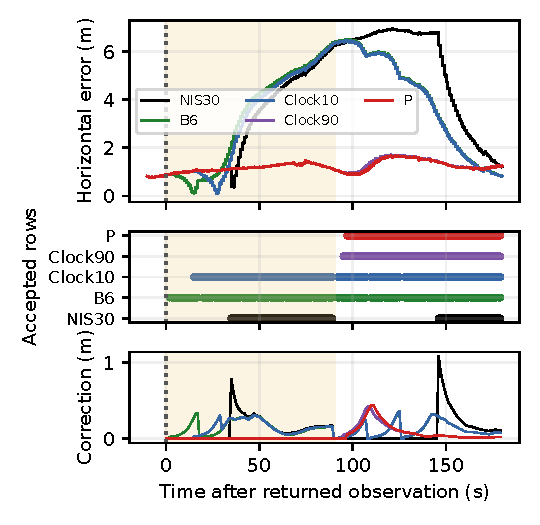
\includegraphics[width=\columnwidth]{figures/first_registered_bias_event.pdf}
\caption{First registered building01 biased event, fixed by order rather than winning margin. Shading is the 90-s injection. Position error, accepted rows and update corrections are distinct. NIS30, B6, Clock10/90 and P are predetermined comparators.}
\label{fig:event}\end{figure}
P's complete biased-event record is:event 0: 1.1667 m, first update 97 s, 0/90 injected rows; event 1: 3.4131 m, first update 7 s, 83/90 injected rows; event 2: 2.5555 m, first update 7 s, 83/90 injected rows. The first event in Fig.~\ref{fig:event} was specified before precision access. These actual biased admissions cannot be inferred from clean latency or silently removed from macro averages. In the three independent biased intervals, injected displacement reduces the offline initialization-conditioned raw receiver error for 44 of 270 rows. Exposure therefore cannot be converted into actual fault probability. All seven categories, extended windows, individual event errors, P95/Max and censored policies are retained in machine-readable tables; no best-event subset determines the main statistic.

\subsection{Seen Evidence and Cross-Route Judgment}
On the primary seen building00 cache, P has 7-s clean admission and 3.0222-m bias90 versus Clock10's 15 s and 5.3611 m; Clock90 has 95 s and 2.5098 m. The second cache has 2.8837-m P bias90 and 2.0854-m Clock90. On seen parking00, NIS30 has 0-s admission and 2.0234 m, versus P's 7 s and 2.2901 m. Removing decay gives 2.2587 m there, slightly below P. Those stronger simple controls and the original R1\texttt{NO\_ADDITIONAL\_GAIN} conclusion remain visible. The old building-route percentage is not presented as an independent-route improvement. The separate native KF-GINS transfer, fixed at the R1-selected noise STD multiplier 2, gives 17.10m natural horizontal RMSE with 1.000 coverage. It is a transferred GNSS/INS configuration, not its best possible accuracy and not a denominator for P's gain.

\section{Discussion}
The prospective route does not support the preregistered joint claim: biased-return error decreases, but the natural-cost cap is violated. The evidence is a conditional tradeoff and failure boundary, not a compliant superiority claim. The new route is one fixed, descriptive replication rather than a sample of deployment environments. Within-route events are correlated; no IID significance or calibrated fault probability is inferred. The normal-cost gate is an explicit application requirement, not permission to hide an excluded strict-NIS result. Long waiting may protect finite biased intervals at the cost of timely clean correction. Relaxing the budget can change the strongest alternative; all registered sensitivity budgets are reported without replacing the primary 15-s protocol.

The manager cannot resolve all local drift and GNSS bias, and correlated raw-GNSS/LIO anchors lack a rigorous independence model. Fallback admits unresolved observations, not certified correct data. Shared MM/INS sensing, known initialization and fixed alignment restrict transfer. The earlier identical-input frontend discrepancy remains unresolved, with 9.7876-m maximum difference; no concurrency cause is established and no favorable cache is selected. Native timing is processing through incremental mapping, excluding preprocessing/publication/wait; Python cached replay excludes frontend and deployed transport. None of these timings establishes field end-to-end real-time performance.

The evidence supports an empirical, scope-limited review manuscript. It does not automatically establish algorithm novelty, a new mechanism increment or readiness for formal submission. Authors must assess whether the full-paper empirical contribution or a shorter abstract is appropriate; acceptance is not guaranteed by execution or small numerical gains.

\section{Conclusion}
GNSS availability, actual update delay, injected-row exposure and position error are separate endpoints. A pushed prospective freeze and complete new-route matrix make the timeliness--accuracy question reviewable without post-test tuning. The prospective route does not support the preregistered joint claim: biased-return error decreases, but the natural-cost cap is violated. The evidence is a conditional tradeoff and failure boundary, not a compliant superiority claim. Stronger controls, all fixed events and retained failure cases are part of the result.

\section*{Reproducibility and Acknowledgments}
Source/configuration hashes, raw/cache identities, freeze and remote receipts, complete tables, vector plot points and independent checks are retained on the authorized separate S8 branch. Raw bags, runtime and full trajectories remain local; Git is a partial evidence backup. Data are used under the dataset's stated academic terms. No author names, affiliations, funding, copyright or formal submission have been assigned or performed. The current PDF is an author-review version; exact venue template variant, anonymity, cutoff/timezone and AI-policy applicability require confirmation.

OpenAI Codex (GPT-6) assisted orchestration, evaluation and plot code, evidence organization and manuscript drafting across the abstract and all text sections. Methods report the recorded execution and independent verification; numeric plots use retained experimental data rather than synthetic artwork. Human authors must verify scientific interpretation, code, references and wording before adoption. This disclosure does not substitute for author responsibility or venue-specific requirements.
\bibliographystyle{IEEEtran}\bibliography{references}
\end{document}
